\documentclass[../main.tex]{subfiles}
\usepackage{silence}
\WarningFilter{glossaries}{No \printglossary or \printglossaries found}
\robExtConfigure{disable externalization}
\begin{document}
\ifSubfilesClassLoaded{%
	\graphicspath{{figures/8-Conclusions/}}%
	\setcounter{chapter}{7}%
	\mainmatter%
}{
	\graphicspath{{../figures/8-Conclusions/}}%
}
\chapter{Conclusions and Perspectives}
\minitocpage
\section{Conclusions}
	During this PhD,
	context precision medicine, focus on omics data, high dimensional
	task diagnosis/prognosis
	fully recap biological process use all information, multi level
	explored the interest of attention on omics data
	In~\cref{chap:attomics}, interest of attention
	groups, memory requirments, introduce knowledge to construct the groups
	AttOmics leverages self-attention to capture feature interactions specific to each patient.
	less parameters but still project in high dim, avoid large compression of the info
	The self-attention also allows the visualization of the learned interactions to understand the model better.
	\textcolor{red}{AttOmics is the only architecture consistently performing well on different omics data.}
	In~\cref{chap:crossattomics}, multi-omics based on the known regulatory interactions at the modality level.
	architecture briefly
	For instance, DNAm impact the level of
	pretrained encoders, boost perf, exchange information in very limited data settings
	CrossAttOmics harnesses cross-attention to build a multimodal representation that explicitly considers interactions between modalities.
	CrossAttOmics outperforms other deep learning architectures when there are very few paired training examples.
	This is achieved by allowing information to flow between the different omics through the cross-attention layers.
	By explicitly modeling the interactions between different omics, attribution methods such as \gls{lrp} can help in identifying the most important interactions.
	Instead of scoring the interactions with post-hoc methods, let the network directly score with a gating mechanism.
	interpretable model !
	CrossAttOmicsGate, score the interaction --> let the network focus on the important interactions
	Gate importance scores must be sparse to ensure correct interpretability and diversity to reflect the diversity that exists between samples.
	To ensure these two properties are met, we added four regularization terms to our training process.
	Our ablation study showed that the four terms are essential to ensure both sparsity and diversity while improving accuracy.

	interpretability important, high-stakes domain such as healthcare, understand why/how a prediction was made, ie what were the important features.
	knowing what are the important features helps knowing what we should change to have a different prediction.
	counterfactuals, use them to know which needs to be made on the expression profile for the patient to be healthy, by linking this perturbation to drug database, provide treatment recommendation.
	consider robust model, adversarial

\section{Perspectives}
	This section aims to expand on the work described in this manuscript and discuss broader perspectives related to the precision medicine field.
	\subsection{Removing groups in AttOmics}\label{sec:scalar_attention}
		In \cref{chap:attomics}, we introduced AttOmics an architecture based on the self-attention mechanism.
		To avoid self-attention limitations on high-dimensional vectors, we proposed to group features and apply the attention mechanism to these groups.
		While this approach was shown to be effective~(\cref{chap:attomics}), groups are an architectural constraint; removing them would allow for directly considering feature interactions.
		However, the self-attention operation requires elements with an embedding dimension strictly greater than one, since elements of omics profiles are scalar values with no embedding dimension an intermediate transformation is required.
		The direct idea would be to project scalar values into a higher dimensional space and use the recent self-attention approximation~\cite{xiongNystrOmformerNystr2021,Linformer} or new efficient implementation~\cite{FlashAttention,rabeSelfattentionDoesNot2021,bolyaHydraAttentionEfficient2022a} that allows for scaling up to large inputs\footnote{see~\cite{EfficientTransformers} for an extensive overview of the possible methods}.
		Nevertheless, there is no justification for projecting scalar values into a higher space, and more importantly, it is unclear what would represent each dimension of the newly obtained vector.

		The attention matrix is obtained by measuring the similarity between pairs of inputs, for vectors this measure is the scalar product.
		One could consider a similarity measure for scalar values, such as absolute difference, and inject this in the attention computation:
		\begin{equation}
			A_{ij} = \operatorname{softmin}\left(\left|Q_{i} - K_{j} \right| \right) \label{eq:scalar_attention}
		\end{equation}
		where \(Q_{i}\) is the \(i\)-th value in the query vector and \(K_{j}\) is the \(j\)-th value in the key vector\footnote{Note that query, key and value are no longer matrices but vectors.}.
		\pythoncode[label={code:torch_att}]{Pytorch implementation of the ScalarAttention}{figures/8-Conclusions/ScalarAttentionPyTorch.py}
		This scalar formulation of the self-attention~(\cref{eq:scalar_attention}) can be easily implemented in PyTorch~(\cref{code:torch_att}) and has already been tested in~\cite{Lacan2023} but still requires to compute and store large \(d\times d\) attention matrices~(\cref{fig:lin_attention_benchA}).
		\citeauthor{Lacan2023} masked the attention matrix and only computed attention for features pairs known to be interacting (\gls{ppi})\cite{Lacan2023}.
		The \(i\)-th element of the attention output is computed as the scalar product of the \(i\)-th row of the attention matrix with the value vector, and the \(i\)-th row of the attention matrix corresponds to the absolute difference of the query vector with the \(i\)-th value of the key vector.
		\begin{equation}
			Z_{i} = \left| Q - K_{i} \right| \cdot V
		\end{equation}
		This formulation can be implemented in an optimized triton kernel~\cite{TritonLang} as proposed in~\cref{code:triton_att}, with a lower memory footprint withtout significantly increase the computation time~(\cref{fig:lin_attention_bench}).
		\pythoncode[label={code:triton_att}]{Triton implementation of the ScalarAttention}{figures/8-Conclusions/ScalarAttention.py}

		\begin{figure}[htbp]
			\centering
			\begin{subcaptiongroup}
				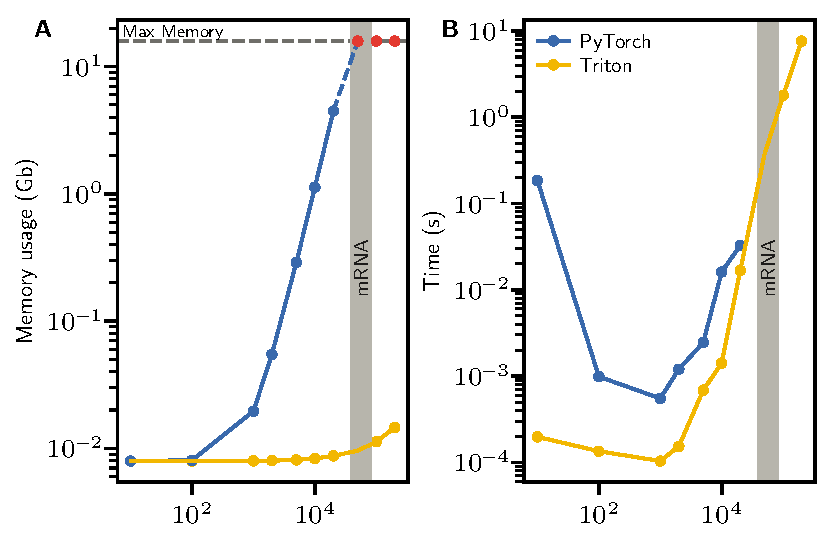
\includegraphics{ScalarAttentionBenchmark.pdf}
				\phantomcaption\label{fig:lin_attention_benchA}
				\phantomcaption\label{fig:lin_attention_benchB}
			\end{subcaptiongroup}
			\caption[Comparison of two ScalarAttention implementation]{Comparison of the memory usage~\subref{fig:lin_attention_benchA} and the computation time~\subref{fig:lin_attention_benchB} of a \textcolor[HTML]{3969AC}{PyTorch} and a \textcolor[HTML]{F2B701}{Triton} implementation of the ScalarAttention}
			\label{fig:lin_attention_bench}
		\end{figure}

	\subsection{Extending CrossAttOmics to other type of modalities}
		In \cref{chap:crossattomics}, we introduced CrossAttOmics a deep learning architecture to integrate multi-omics data.
		As the attention mechanism can adapt any type of modalities, such as text or images, with the correct dimensions, a natural extension would be to consider non omics modalities such as histopathology images, clinical information or textual reports.
		The main question would be how to connect them with the rest of the omics interactions graph~(\cref{fig:tcga_graph}).
		Furthermore, the ScalarAttention proposed in \cref{sec:scalar_attention} can be extended to multimodal context, \ie{}a CrossScalarAttention where the query comes from one modality and the key from another one.
		Using such an attention mechanism would refine the considered interactions to the feature level.
		A modality interaction graph would define on which modality pairs the cross-attention is computed and the cross-attention matrix could then be masked or regularized\footnote{see discussion on knowledge integration in \cref{sec:persp_knwoledged}.} to focus on direct relation ships.
		For instance an \gls{mirna} is expected to only interact with its \gls{mrna} targets\footnote{some \gls{mrna} targets are experimentally verified and other are putative targets based on the sequence complementarity.}.

	\subsection{Biological knowledge}\label{sec:persp_knwoledged}
		Biolgically-informed architectures are common when applying deep learning to biological problems as they provide a strong inductive bias.
		However, adding knowledge into the deep learning architectures is challenging as they are things that are still unknown\footnote{This is probably more a philosophical question to know whether we have a complete understanding of the biological mechanism or if there is still some to be discovered.}.
		For instance, annotations mainly cover coding genes, but noncoding genes are known to be involved in gene expression regulation.
		Focusing only on annotated genes would leave out many features\footnote{For instance in \gls{go} only XX \gls{ncrna} are annotated} and limits model capacity to consider all interactions, which at the end might limit the predictive performances.
		Moreover, excluding unannotated features prevents researchers from discovering new biomarkers that could be detected by training models on all available features.
		Instead of excluding unannotated features, a regularization favoring knwon relationships could be added to the training objective.
		This kind of approach allow to exploit knowledge while allowing the network to use unannotated features and potentially discover new features interactions.

		Another aspect of knowledge integration is the continual construction of our understanding of biological mechanisms; some things we consider true become invalid, and newly discovered things enrich our knowledge.
		This means that a model constructed at time \(T\) might become invalid at time \(T+1\) because our knowledge has evolved.
		Models would have to be retrained to incorporate up-to-date knowledge, but constantly retraining models can be economically and environmentally costly.
		Continual learning might provide opportunities to develop AI systems that can continually acquire and update their knowledge\cite{wang2024comprehensivesurveycontinuallearning}.

	\subsection{Omics data challenges}
		Omics data are generated with various methods, various sequencing platform, at different places and time by different people.
		Those variations leads to non-biological variation in the data, also knwon as \emph{batch effect}~\cite{Leek2010}.
		Deep learning models are sensitive to batch effects as they might capture and amplify those artifacts.
		Model interpretability can help to detect such cases, but there is still a need to better consider batch effect by correcting it or adding domain adaptation tasks to ensure the same representation of all samples.
		Moreover, various tools have been developped to extract gene counts from sequencing reads and might leads to different outputs.
		The generated gene counts can also be impacted by the choice of the reference genome.
		It is important to ensure that all samples have been analyzed in an identical way with fixed references.
		There is a need of more initiative like \glsxtrshort{tcga} or ARCHS4~\cite{Lachmann2018} to provide data that have been analyzed with a common pipeline.

		\Gls{tcga} is an ongoing project regularly updated with new releases\footnote{\url{https://docs.gdc.cancer.gov/Data/Release_Notes/Data_Release_Notes/}} that add new data or correct erroneous information, which makes it more difficult to fairly compare various approaches since they are likely using different versions with various subset of included cancers.
		This highlights\footnote{along with the non sharing of model weights, and in worst cases the absence of source codes} the need for a standardized benchmark to fairly compare multiple approaches.

		While the development of high-throughput sequencing methods increased the availability of omics data, the number of available samples remains limited compared to other deep learning fields.
		Moreover, when analyzing multi-omics data, gold standard datasets where all modalities are available for all samples are rare.
		Datasets where some modalities are available for some patients are more common as generating all modalities will increase the cost or the patient did not accept some analysis.
		This results in datasets with various missingness patterns where two different samples have different set of available omics.
		Such datasets are challenging to use with deep learning multimodal architectures.
		In \cref{chap:crossattomics}, we proposed to simulate the various missingness pattern during the training which increased the robustness to missing modalities.
		Although this approach was effective, it increased the training time and supposed that all missingness pattern are generated during the training phase.
		Another way would be to generate the missing modalities from the other modalities using a generative or modality translation task.
		Generating large molecular profile is still a difficult task as such network are difficult to train.
		Other methods handling missing modalities project the available ones in a common latent space before combining\footnote{linear combination, product of experts, \dots} them; such model are trained in a self-supervised fashion~\cite{Lee2021AVI}.
		%TODO: Figure how to handle missing modalities 

	\subsection{single-cell}
		applied on bulk-experiments
		diagonal integration

	\subsection{Foundation models}

		https://www.science.org/doi/10.1126/science.abc4552

		Lung Cancer Subtype Diagnosis using Weakly-paired Multi-omics Data~\cite{Wang2022}
		subtype; miRNA, SNV, DNAm, WSI
		IF
		encode each omics individually with an attention based encoder
		how are obtained the attention weight ??
		from latent representation, predict the subtype (first loss component)
		how they handle missing omics: GAN based on the combination of the available modalities

\end{document}
